\documentclass[12pt,a4paper]{article}
\usepackage[protrusion=true,expansion=true]{microtype}
\linespread{1.3}

\usepackage{float}
\usepackage{amssymb}
\usepackage{caption}
\usepackage[utf8]{inputenc}
\usepackage[T1]{fontenc}
\usepackage{graphicx}
\usepackage[bookmarks=true,hidelinks=true,breaklinks=true]{hyperref}
\usepackage{mathptmx}
\usepackage{cleveref}
\usepackage{enumitem}
\usepackage{minted}
\usepackage[backend=biber,natbib=true,style=apa]{biblatex}
\usepackage[scaled=.92]{helvet}
\bibliography{references.bib}

\begin{document}
\title{Der Transparente Mensch: Die unvermeidliche Preisgabe von Metadaten }
\author{Arne Beer, MN 6489196, University of Hamburg}
\date{20.08.2019}

\maketitle


\section{Abstract}

Metadaten spielen eine bedeutende Rolle in der Welt der Datenanalyse.
Simple Informationen über einen Menschen, wie zum Beispiel der Standort verknüpft mit Zeitpunkten, verschiedene Aktivitäten oder Vorlieben, liefern enormes Potential, um diesen zu analysieren und kategorisieren.
In vielen Fällen wird aktives Sammeln von Daten, Data Mining und Big Data Analysis betrieben und Plattformen wie Facebook, haben sich voll diesem Ziel verschrieben.

Metadaten sind jedoch tückisch und befinden sich an viel mehr Orten als man vielleicht auf den ersten Blick vermutet.

Dieses Paper wird sich speziell mit der Intransparenz in Bezug auf die Freigabe von Metadaten bei bestimmten Tools auseinandersetzen, welche eigentlich nicht für diesen Zweck vorgesehen sind.
Speziell betrachten wir in diesem Falle das Tool \emph{Git}, welches hauptsächlich zur Versionskontrolle von Quellcode in Informationstechnischen Projekten verwendet wird.
Zudem wird die populäre Website \emph{GitHub} betrachtet, welche als Open-Source Plattform dient, auf der jeder Entwickler seine Projekte öffentlich zur Verfügung stellen kann.

\newpage

\section{Einleitung}
Das Ziel dieser Arbeit ist, die Notwendigkeit von Datenerfassung zu betrachten.
In einigen Umfeldern, speziell im Informationstechnischem Bereich, ist die Erfassung von Metadaten unvermeidlich und teilweise unabdingbar.
Daten werden zur Analyse von technischen Prozessen benötigt oder um z.B. die Verantwortlichkeit eines Entwicklers für eine bestimmte Änderung an einem System festzuhalten.

Leider lassen sich aus simplen Metadaten jedoch häufig mithilfe von Data Mining Techniken mehr Informationen als auf den ersten Blick ersichtlich.
Hierbei kann es dazu kommen, dass durch simple Hilfsmittel, welche lediglich die Produktivität und Benutzbarkeit eines Werkzeugs verbessern sollen, private Informationen über den Nutzbar nach außen hin ersichtlich werden.
Falls diese Daten nun zusätzlich öffentlich einsehbar sind, können diese von einer nicht kontrollierten Instanz benutzt werden.

Aus diesen Umständen entsteht ein Dilemma, welches aus dem Konflikt zwischen der Notwendigkeit Daten zu erheben und zu veröffentlichen und der unmöglichen Kontrolle über die Verbreitung dieser Daten besteht.
Im Folgenden wird dieses Problem in Bezug auf Privatheit und Transparenz am Beispiel der professionellen Open-Source Community und dem Tool Git näher betrachtet.

\section{Git und Github}
Diese Arbeit erläutert die vorliegende Problematik am Beispiel des Tools \emph{Git} und der Plattform \emph{GitHub}.
Hierzu werden im Folgenden die beiden Technologien vorgestellt, wichtige Aspekte erörtert und zusammengefasst.


\subsection{Git}
Git ist ein heutzutage als Standard angesehenes Werkzeug zum Entwickeln von Projekten im Informationstechnischen Sektor.
Beinahe jedes Projekt mit Quellcode besitzt eine Art von Version Control System (VCS), und in den meisten Fällen wird diese Rolle von \emph{Git} eingenommen.
Ein VCS ist ein Hilfsmittel, welches es erlaubt den Quellcode zu versionieren, also zu bestimmten Zeitpunkten eine Version des momentanen Standes des Projekts festzuhalten.
Ein Projekt, welches von Git verwaltet wird, wird im Fachjargon ein \emph{Repository} genannt.

Durch diese Versionierung, ist es den Entwicklern des Projekts möglich schnell zwischen verschiedenen Versionen hin und her zu wechseln.
Sollte also zum Beispiel ein neues Feature einer Software fehlerhaft sein und nicht funktionieren, kann mithilfe eines Befehls ohne weiteren Aufwand zu der vorherigen stabilen Version des Projektes gewechselt werden.
Eine solche Version wird in Git als \emph{Commit} bezeichnet.
Ein \emph{Commit} kann nun wiederum auf einen oder mehrere andere \emph{Commits} zeigen, welche die \emph{Parents}, also deren Vorfahren, bezeichnet werden.

Wenn ein neuer \emph{Commit}, also eine neue Version, erstellt wird, zeigt dieser also immer auf die vorherige Version, von der dieser abgeleitet wurde.
Durch diese Verbindung zwischen den \emph{Commits} lässt sich folglich die komplette Historie des Projektes ableiten und zu jedem Zeitpunkt des Projektes zurückspringen.
Diese Struktur wird in Git die \emph{History} genannt, welche man als gerichteten azyklischen Graphen darstellen kann.

\begin{figure}[H]
    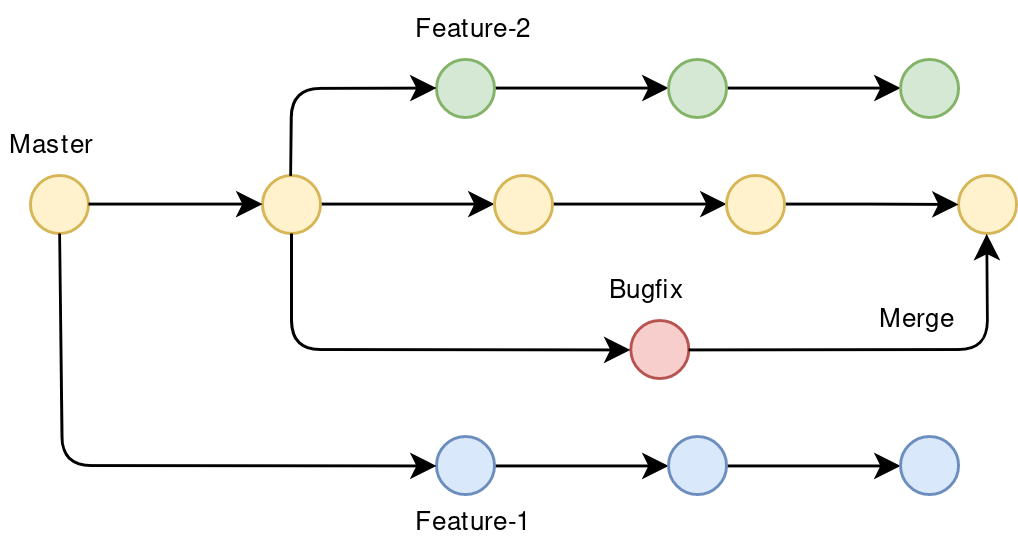
\includegraphics[scale=0.25]{./gfx/git-history-branch.png}
    \centering
    \caption{Eine beispielhafte Darstellung einer möglichen \emph{History} in Git.}\label{fig:git-history}
\end{figure}

Wenn man sich nun jedoch einen solchen \emph{Commit} genauer anschaut, fallen einige sehr interessante Details auf.
In Listing~\ref{lst:raw-commit} kann die Struktur einer solchen Datei gesehen werden und es sind mehrere direkte Identifikatoren und Metadaten zu sehen.
Zum einen ist der volle Name und die Email Adresse ersichtlich, welche vermutlich zu einer vollständigen Identifikation ausreichen würden.
Zudem ist Timestamp mit dem momentanen UTC Offset des Erstellers des \emph{Commits} eingebunden.

\begin{minted}[linenos]{text}
    tree      cd7d001b696db430b898b75c633686067e6f0b76
    parent    c19b969705e5eae0ccca2cde1d8a98be1a1eab4d
    author    Arne Beer <test@eintest.de> 1513434723 +0100
    committer Arne Beer <test@eintest.de> 1513434723 +0100

    Chapter 2, acronyms
\end{minted}
\begingroup
\captionof{listing}{Eine Git \emph{Commit} Datei. Auf unterster Ebene wird ein \emph{Commit} nur durch eine Textdatei in diesem Format dargestellt.\label{lst:raw-commit}}
\endgroup

Es ist folglich für jede neue Version zu sehen, wer diese erstellt hat, wann er sie erstellt hat und in welcher Zeitzone sich diese Person zu diesem Zeitpunkt aufgehalten hat.
Ebenfalls verbunden mit einem Commit sind alle Änderungen, die der Autor zwischen dieser und der letzten Version vorgenommen hat.


\subsection{GitHub}
GitHub ist die zur Zeit größte Open-Source Plattform mit über 96 Millionen öffentlichen Repositories.
Es ist eine Seite, die zur Verbreitung von Wissen, öffentlicher Software, zum Lernen sowie zum entwickeln kommerzieller Projekte verwendet wird.
Neben dem bloßen Bereitstellen einer Plattform, werden zudem Tools angeboten, welche die Kollaboration zwischen Entwicklern vereinfacht.
Dadurch wird die Hürde zum Beitragen an fremden Projekten deutlich gesenkt und dementsprechend sogar Kollaboration gefördert.

Github ist jedoch nicht einfach nur eine Plattform zum Verteilen von freier Software, sie wird ebenfalls benutzt um sich selbst als Entwickler zu profilieren.
Viele Software Developer partizipieren in der Erstellung oder Weiterentwicklung von Projekten aus Leidenschaft heraus, allerdings jedoch auch mit dem Wissen, dass diese Beiträge ihr Resume darstellen und dadurch direkten Einfluss auf den Marktwert ihrer Fähigkeiten hat.

Zudem bietet Github einige Features, die an Funktionalitäten aus größeren Social-Media Plattformen erinnern.
So erlaubt Github es seinen Nutzern Sterne zu vergeben, wenn ihnen ein Projekt gut gefällt.
Diese Sterne werden zudem gerne als Maßstab für den Erfolg und die verbreitete Nutzung eines Projektes verwendet.

\section{Transparenz}

Dieser Abschnitt befasst sich mit dem Begriff der Transparenz in Bezug auf das Tool Git und die Plattform GitHub.
Transparenz wird hier in zwei verschiedenen Konnotationen benutzt werden.
Zum einen wird überprüft in wie weit die Veröffentlichung von Metadaten transparent dargelegt wird.
Zum anderen wird untersucht, in wie weit der Zugriff und die Verbreitung der veröffentlichten Daten verboten oder zugelassen wird.

\subsection{Benutzung}
Der Begriff der Transparenz in Bezug auf die Nutzung von Git, bezieht sich in erster Linie darauf, ob klar kommuniziert wird, dass potentiell persönliche Daten veröffentlicht werden und falls ja, welche Art von Daten veröffentlicht werden.

Hier spielt die Komplexität eines Programmes eine große Rolle.
So wird es zunehmend schwerer die Auswirkung einer Handlung abzuschätzen, speziell mit der zunehmenden Komplexität des unterliegenden Programms (\cite[p. 2]{article:dataethics}).

Git wird in erster Linie als Commandline Tool verwendet.
Hierbei werden bestimmte Befehle auf der Konsole eingegeben, welche interpretiert werden und anschließend die gewünschte operation ausführen.
Die Tatsächlichen Metadaten, die bei diesen Operationen erstellt werden, sind beim alltäglichen Gebrauch nicht ersichtlich und meist nicht notwendig für die Benutzung des Programms.
Daher wird häufig nicht über diese aufgeklärt.
Für interessierte Entwickler, gibt es ein öffentliches Buch, welches genauer auf die unterliegenden Funktionalitäten und Methoden von Git eingeht, jedoch ist dieses wie bereits gesagt keine notwendige Lektüre (\cite{book:pro-git}).

Auch bei dem weiteren Durchsuchen der offiziellen Hilfe Seite von Git, findet sich keine Hinweis oder Warnung darüber, dass Daten nach außen hin veröffentlicht werden könnten (\cite{online:manpage}).

Es wird offensichtlich nicht klar kommuniziert, welche Daten von Entwicklern aufgezeichnet werden und wie diese potentiell missbraucht werden könnten, wenn sie an die Öffentlichkeit gelangen.


\subsection{Kontrolle}
Die Analyse von Personenbezogenen Daten, kann zu einer Menge an Informationen über die verschiedenen Interessen, Herkunft, Erfahrungen einer Person ergeben (\cite[p.~4-5]{article:corporate}).
Im Kontext von Git und GitHub, wird schnell ersichtlich, dass durch die Veröffentlichung von Git Repositories, eine Menge an persönlichen Daten freigegeben wird.

Die volle Transparenz eines Nutzers kann große Nachteile nach sich ziehen, besonders wenn der Nutzer sich nicht direkt klar über die Ausmaße der Transparenz ist.
Wenn ein System ohne eine klaren Vorstellung implementiert wird, in welcher klar geregelt ist, warum welche Daten veröffentlicht werden sollten, kann die Transparenz die Privatsphäre des Nutzers bedrohen (\cite[p.~6]{article:seeing-knowing})

GitHub stellt eine API zur Verfügung, die es erlaubt die Website programmatisch zu erkunden und mit dieser via Code zu interagieren.
Durch diese API ist es möglich mit mit relativ guter Präzision die meisten Repositories zu der eine einzelne Person oder eine Gruppe von Personen beigesteuert hat, zu finden und von diesen Daten zu extrahieren (\cite[p.~14-16]{thes:thesis}).

Es herrscht kein wirklicher Mechanismus um großflächiges Sammeln von Daten zu verhindern und es existieren sogar bereits Projekte, wie zum Beispiel GHTorrent, welche alle Daten von Github live beobachten und jedem öffentlich zur Verfügung stellen.
Dadurch kann jeder, auch Personen ohne größeres technisches Verständnis, diese Daten herunterladen und benutzen.

Durch Daten dieser Art, ließ sich zum Beispiel eine großangelegte Studie durchführen, ob Software Entwickler in den Mozilla Open-Source Projekten eher während der Nacht oder am Wochenende entwickeln (\cite{inproc:work-night}).

Jedoch lassen sich diese Analysen nicht nur auf eine Gruppe von Personen anwenden, sondern auch auf eine Einzelperson.
So war es zum Beispiel möglich mithilfe von Github gewonnenen Daten sehr präzise die Urlaubs und Krankheitsausfälle mehrerer Arbeiter eines Unternehmens zu analysieren (\cite[p.~37-39]{thes:thesis}).

Wenn nun weitere Daten von GitHub eingebunden werden, könnte ein sehr genaues Profil eines aktiven Entwicklers erstellt werden, welches die Schlafzeiten, Krankheitsausfall, beherrschte Technologien, die Erfahrungen mit einer bestimmten Technologie und Produktivität umfassen könnte.

Ein solcher Datensatz wäre beispielsweise perfekt geeignet um gezielte Rekrutierungen von Entwicklern mit einem bestimmten Skill Set durchzuführen.

Ebenfalls ist vorstellbar, das durch die Analyse von Repositories Mitarbeiterüberwachung durchgeführt werden kann.
Durch die Anzahl der Commits und die Länge und Qualität des hinzugefügten Codes könnte die Effizienz eines Mitarbeiters bestimmt werden und Mitarbeiter, welche eine bestimmte Quota nicht erfüllen, könnten Opfer einer Benachteiligung werden.
So existieren bereits mehrere Methoden, um die Effizienz eines Entwicklers anhand von geschriebenen Zeilen von Code zu berechnen (\cite{inproc:measuring-loc}).

Wie z.B. die Snowden Enthüllung gezeigt hat, werden Daten heutzutage im großen Stil gesammelt, von den verschiedensten Quellen und sie werden auf auf bisher nie dagewesene Arten miteinander verbunden und auf neue Weisen angewendet (\cite[p.~4]{article:snowden}).
Eine Anwendung zur Analyse von Git repositories und Github im professionellen Sektor ist nicht unrealistisch und höchstwahrscheinlich schon vorhanden.


\subsection{Privatheit}

Um die Auswirkung auf die Privatsphäre einer Person, betrachten wir hierzu zuerst eine Definition der Privatsphäre von W.A. Parent.

\begin{quote}
Privacy is the condition of not having undocumented personal knowledge about one possessed by others. A person's privacy is diminished exactly to the degree that others possess this kind of knowledge about him.
Documented information is information that is found in the public record or is publicly available (e.g.~information found in newspapers, court proceedings, and other official documents open to public inspection) (\cite[p.~203]{paper:privacymorality}).
\end{quote}

Mit dieser Definition und dem Wissen aus dem vorherigem Abschnitt, lässt sich erschließen, dass wir es in unserem Fall mit dokumentierter Information haben.
Zudem handelt es sich um volle Transparenz in Bezug auf die veröffentlichten Projekte und die Arbeitszeiten und Fähigkeiten des Nutzers.

Der Nutzer hat zwar stets die Möglichkeit seine Projekte zu verbergen oder erst gar nicht auf GitHub oder einer anderen Seite zu veröffentlichen, jedoch würde dies gegen das Grundsätzliche Prinzip von Open-Source sprechen.
Der gesamte Sinn hinter GitHub ist, eine Plattform für die freie Verbreitung von Wissen zu bieten, welches ein nobles moralisch wünschenswertes Ziel ist.

\section{Diskussion}

Within the discourse of computer science, transparency is often seen as desirable because it brings insight and governance (\cite[p.~6]{article:seeing-knowing}).

\section{Zusammenfassung}


In dieser Arbeit wurden zudem nur die Aspekte der Transparenz und der Privatheit angesprochen.
Jedoch sollte ebenfalls die Fairness und Sauberkeit der Daten berücksichtigt werden.
Git Repositories haben selten eine komplett saubere und nachvollziehbare History.
Commits können beispielsweise bearbeitet, gelöscht, überschrieben und zusammengefasst werden, um nur ein paar der Möglichen Fehlerquellen zu nennen.
Durch diese Fehlerquellen könnten Analysen verzerrt werden.
Die Errungenschaften einer Person könnten versehentlich auf eine andere übertragen werden und ungerechtfertigte Benachteiligungen oder Anschuldigungen wären die direkte Folge einer solchen Analyse.

\section{Literatur}

\printbibliography
\end{document}
